\section{System Overview}
\label{sec:fdsp-tpcelec-overview}

%%%%%%%%%%%%%%%%%%%%%%%%%%%%%%%%%%%
\subsection{Introduction}
\label{sec:fdsp-tpcelec-overview-intro}

%%%%%%%%%%%%%%%%%%%%%%%%%%%%%%%%%%%
\subsection{Design Considerations}
\label{sec:fdsp-tpcelec-overview-design}

%%%%%%%%%%%%%%%%%%%%%%%%%%%%%%%%%%%
\subsection{Scope and Requirements}
\label{sec:fdsp-tpcelec-overview-scope}

%%%%%%%%%%%%%%%%%%%%%%%%%%%%%%%%%%%
\subsection{ProtoDUNE-SP Results}
\label{sec:fdsp-tpcelec-overview-pdune}

The Single Phase ProtoDUNE-SP detector, described in Section~\ref{protodune-overview}, is a 700~ton fiducial volume LArTPC with 15,360 sense wires which are read out by a cold electronics (CE) system described in Section~\ref{itf-protodune}. It was deployed in a beamline of the CERN Neutrino Platform in 2018 and continued to take cosmic event data into 2019. The goal for the ProtoDUNE-SP TPC readout was to validate the concept and design of the integrated APA+CE readout and measure the performance of the CE system with components as close as possible to the final DUNE TPC readout.

Each of the six ProtoDUNE-SP APA+CE readout unit consists of 2,560 sense wires, of which 960 are 6.0~meter long collection wires and 1,600 are 7.4~meter long induction wires. Each one was tested in a full scale ``Cold Box'' in cold gaseous Nitrogen (GN2) with a complete CE readout system identical to the one on the detector prior to installation in the cryostat. Figure~\ref{fig:apa2-cycle} shows the Equivalent Noise Charge (ENC), which is the charge in electrons that would have to arrive at the sense wires to generate a signal with the RMS measured by the Front-End electronics, as a function of cold cycle time. At a stable temperature of 160 Kelvin the ENC for all 3 wire planes is below 500~e$^-$.

\begin{figure}
    \centering
    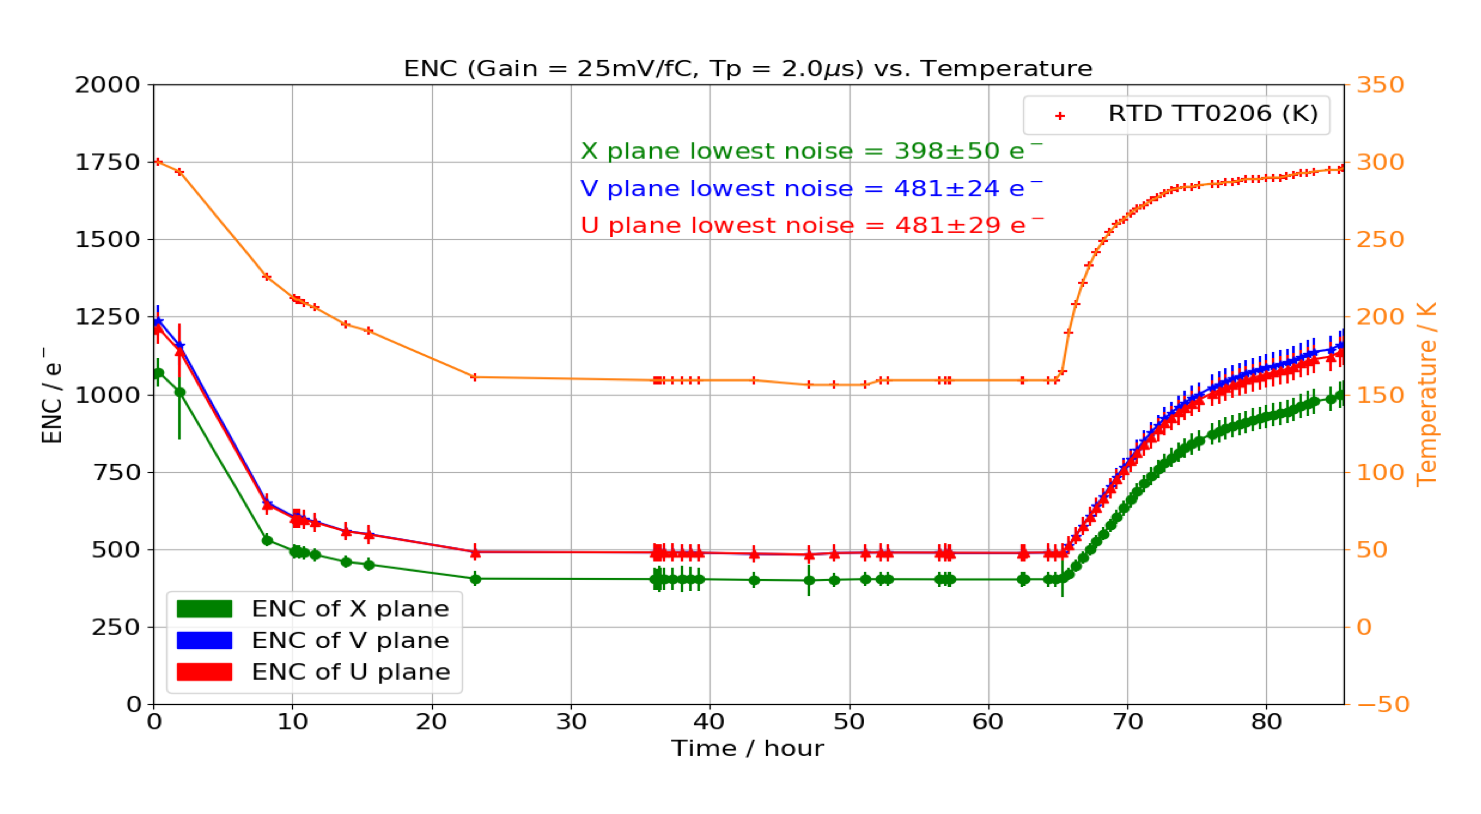
\includegraphics[width=1.0\linewidth]{sp-tpcelec-apa2.png}
    \caption{Left Y-axis: ENC (in electrons) for U, V and X (red, blue and green curves) sense wire planes as a function of time (hours) for the APA2 cold cycle in GN2 in the CERN Cold Box; right Y-axis: temperature (orange curve) measured at the level of the Front-End electronics.}
    \label{fig:apa2-cycle}
\end{figure}

After the cryostat was filled with LAr and the drift and wire bias HV were set to nominal (defined in Section~\ref{protodune-overview}), 99.7\% of the TPC readout channels were alive. The following channels were expected to be unresponsive to charge deposited on the wires:
\begin{itemize}
    \item 4 electronics channels, suggesting a dead channel in the electronics, all on collection wires on three different APAs;
    \item $\sim$35 channels were measured with ENC consistent with no capacitive load on the Front-End (FE) electronics, suggesting an open connection somewhere in front of the CE system, scattered randomly throughout the detector and on all wire planes.
\end{itemize}
With the detector in nominal operating conditions, the ENC was found to be $\sim$550~e$^-$ on the collection wires and $\sim$750~e$^-$ averaged over all operational channels. Figure~\ref{fig:apa3-noise} shows the ENC in electrons for all channels of one of the APA+CE readout units. The collection channels with ENC$>$1500~e$^-$ are caused by an artifact in the generation of cold ADC ASIC used in ProtoDUNE-SP. The channels in all three planes with ENC$<$300~e$^-$ have an open connection somewhere in front of the CE system.

\begin{figure}
    \centering
    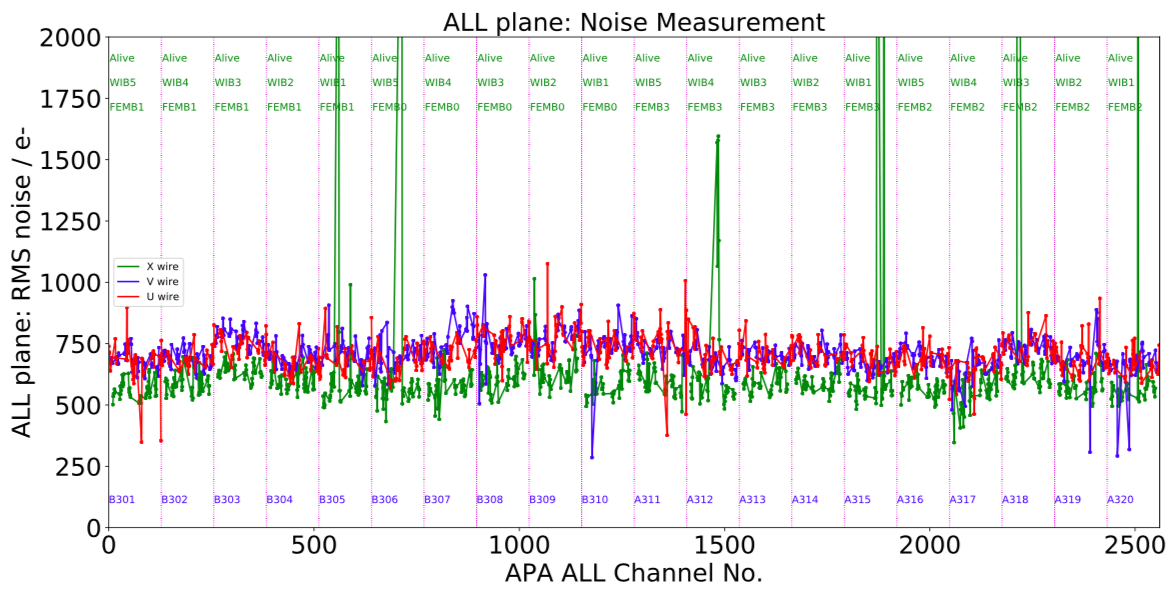
\includegraphics[width=1.0\linewidth]{sp-tpcelec-apa3-enc.png}
    \caption{ENC (in electrons) for all U, V and X (red, blue and green curves) sense wire planes for one ProtoDUNE APA with the detector in nominal operating conditions.}
    \label{fig:apa3-noise}
\end{figure}

The overall performance of the CE system in ProtoDUNE-SP satisfies the DUNE single phase Far Detector CE system requirements listed in Section~\ref{sec:fdsp-tpcelec-overview-scope}. The overall system architecture, described in Section~\ref{sec:fdsp-tpcelec-overview-design}, will remain the same for the DUNE Cold Electronics. However, several improvements and updates to the CE system design motivated by the results from the testing and commissioning of, and the data-taking with, the ProtoDUNE-SP electronics will be discussed in this chapter.
